\documentclass{report}
\usepackage[cmex10]{amsmath}
\usepackage{mathtools}
%\usepackage{txfonts}
\usepackage{wasysym}
\usepackage{hyperref}
\usepackage{amsthm}
\usepackage{mathrsfs}
\usepackage{cite}
\usepackage{cases}
\usepackage{longtable}
\usepackage{enumerate}
\usepackage{enumitem}
\usepackage[nottoc]{tocbibind}
\usepackage[square,numbers]{natbib}
\usepackage{arxiv}
\usepackage{graphicx}
\usepackage[utf8]{inputenc} % allow utf-8 input
\usepackage[T1]{fontenc}    % use 8-bit T1 fonts
\usepackage{hyperref}       % hyperlinks
\usepackage{url}            % simple URL typesetting
\usepackage{booktabs}       % professional-quality tables
\usepackage{amsfonts}       % blackboard math symbols
\usepackage{nicefrac}       % compact symbols for 1/2, etc.
\usepackage{microtype}      % microtypography
\usepackage{lipsum}
\usepackage{subfig}
\usepackage{caption}
\usepackage{subcaption}
\usepackage{csquotes}
\usepackage{listings}
\usepackage{datetime}
%\usepackage{biblatex}
\newcommand{\pasa}{PASA}
\newcommand{\mnras}{Monthly Notices of the Royal Astronomical Society}
\newcommand{\aap}{Astronomy and Astrophysics}
\newcommand{\apjl}{Astrophysics Journal Letters}
\newcommand{\ptrsl}{Philosophical Transactions of Royal Society}

\usepackage[backend=bibtex,style=authoryear-icomp,sorting=ydnt]{biblatex}
\addbibresource{ref.bib}

\captionsetup[figure]{labelfont=it,textfont={it}}
%\captionsetup[subfigure]{textfont=normalfont,singlelinecheck=off,justification=center}

\title{Ice-Cube Data Analysis\\ \textit{B.Tech. Project - Fall 2022}}
\Large
\author{\huge
\onehalfspacing
  Vibhavasu Pasumarti \\\\
  \Large
  EP20BTECH11015\\
  \Large
  Engineering Physics\\
  \Large
  Indian Institute of Technology, Hyderabad \\[1in]
  %\vspace{1in}
  \huge
  \textbf{Supervisor}\\\\
  \huge
  Dr. Shantanu Desai\\\\
  \Large
  Department of Physics\\
  \Large
  Indian Institute of Technology, Hyderabad 
}
\date{\today}
\bibliography{ref}
\begin{document}
\begin{center}

\includegraphics[width=0.75\textwidth]{Images/horzlogolong.png}
\end{center}

\maketitle 

\newpage
%\large
\tableofcontents
\newpage




\begin{abstract}
\large
%\section{OBJECTIVE}
The objective of this project was to determine angular correlation between radio pulsars and ultra-high energy neutrinos using the publicly available IceCube point source neutrino events catalog. For this purpose we use the
unbinned maximum likelihood method to search for a statistically significant excess from each of the pulsars in the ATNF catalog.
\end{abstract}
\newpage
\large
\chapter{\Huge INTRODUCTION}
%\section{\large INTRODUCTION}
\section{Pulsars}
Pulsars are rotating neutron stars, which emit pulsed radio emissions with periods ranging from  milliseconds to a few seconds  with  magnetic fields ranging from $10^8$ to $10^{14}$ G
\section{\large Neutrinos}
Neutrinos are fermionic particles that interact only via \underline{weak interactions and gravity}.
They are electrically neutral and have negligible rest mass.\\
Neutrinos are created by various radioactive decays, some of those  processes which are observed often are:
\begin{enumerate}
    \item Beta decay of atomic nuclei or hadrons
    \item Natural nuclear reactions (such as those that take place in the core of a star)
    \item Artificial nuclear reactions in nuclear reactors, nuclear bombs, or particle accelerators
    \item During a supernova
    \item During the spin-down of a neutron star
    \item When cosmic rays or accelerated particle beams strike atoms
\end{enumerate}
Neutrinos come in 3 \emph{flavours}:
\begin{enumerate}
    \item $e^- $
    \item $\mu$-on
    \item $\tau$
\end{enumerate}
reference https://en.wikipedia.org/wiki/Neutrino

\section{\large Neutrino detection methods}
Due to their negligible rest mass, the gravitational forces exerted by neutrinos cannot be used as a way to detect them. So they are detected with their interactions with matter.\\
Neutrinos interact with matter in two ways
\begin{enumerate}
    \item Neutral current interaction:\\
    \quad In a neutral current interaction, the neutrino enters and transferres some of its energy and momentum to a ‘target’ particle, and leaves the detector. If the target particle is charged and sufficiently lightweight, it might be accelerated to a relativistic speed and consequently emit Cherenkov radiation, which can be observed directly.\\
    However, this detection does not enable us to determine the \emph{flavour} of the neutrino
    \item Charged current interaction\\
    \quad In a charged current interaction, a high-energy neutrino transforms into its partner lepton ($e^-, \mu$, or $\tau$). However, if the neutrino does not have sufficient energy to create its heavier partner's mass, it cannot undergo a charged current interaction.
\end{enumerate}
%\newpage
\section{\large IceCube}
ref:\url{https://icecube.wisc.edu/science/icecube/}
\\
ref:\url{https://en.wikipedia.org/wiki/IceCube_Neutrino_Observatory}\\
The IceCube is a neutrino observatory constructed at the Amundsen–Scott South Pole Station in Antarctica.

\begin{figure}[htbp] % H here makes the images come at the correct position
	\centering
	\begin{minipage}{.5\textwidth}
		\centering
		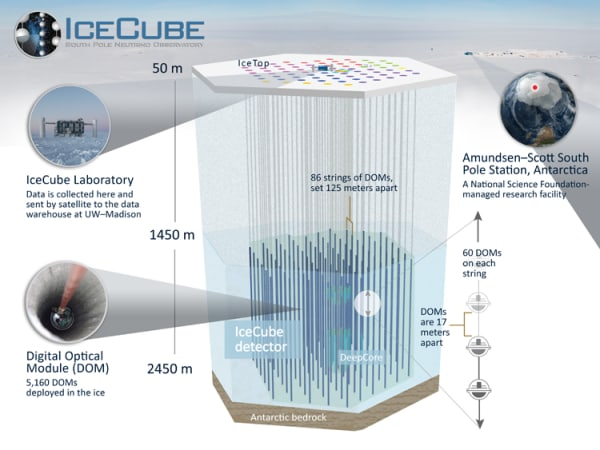
\includegraphics[width=0.8\linewidth]{Images/icecube_detector_schematic.jpg}
		\captionof{figure}{}
	\end{minipage}%
	\begin{minipage}{.5\textwidth}
		\centering
		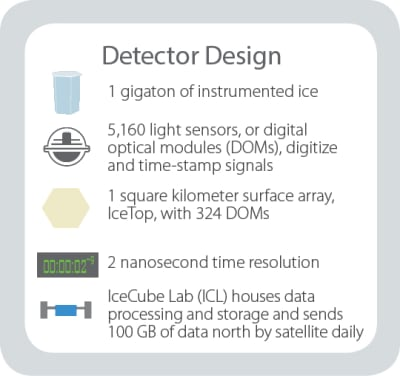
\includegraphics[width=0.65\linewidth]{Images/icecube_detector_design.jpg}
		\captionof{figure}{}
	\end{minipage}
	\caption*{Structure of IceCube Observatory}
\end{figure}
The %in-ice component of 
IceCube consists of 5,160 digital optical modules (DOMs), each with a ten-inch photomultiplier tube and associated electronics. The DOMs are attached to vertical “strings,” frozen into 86 boreholes, and arrayed over a cubic kilometer from 1,450 meters to 2,450 meters depth. The strings are deployed on a hexagonal grid with 125 meters spacing and hold 60 DOMs each. The vertical separation of the DOMs is 17 meters.

\subsection{Working principle}
The IceCube detects neutrinos via the Neutral current interactions. 
When they happen to interact with the ice they produce electrically charged leptons that in turn emit Cherenkov light, as a result of traveling through the ice faster than light travels in ice.

The IceCube sensors collect this light, which is subsequently digitized and time stamped. This information is sent to computers in the IceCube Lab on the surface, which converts the messages from individual DOMs into light patterns that reveal the direction and energy of muons and neutrinos.

When neutrinos (rarely) collide with the molecules of ice, they create charged leptons ($e^-$ $\mu$ons and $\tau$). If the created leptons are energetic enough, they emit Cherenkov radiation which is detected by photomultiplier tubes within the DOMs making up IceCube.

\begin{figure}[htb]
    \centering
    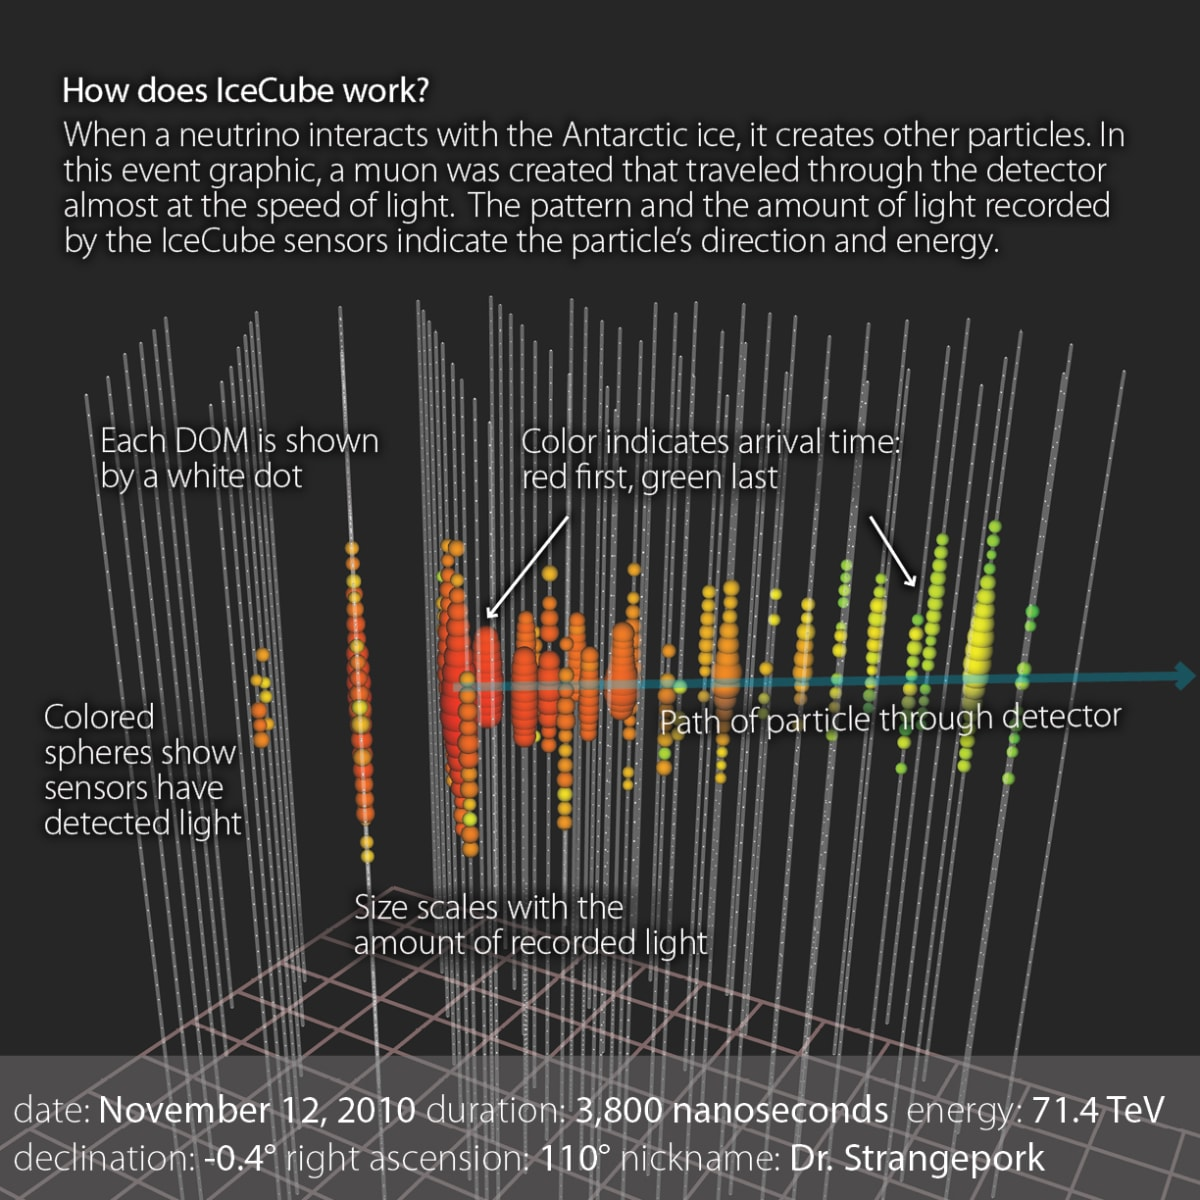
\includegraphics[width=0.5\textwidth,keepaspectratio]{Images/how_does_icecube_work.jpg}
    \caption{Structure of IceCube Observatory}
    \label{fig:IC_schematic}
\end{figure}
IceCube is more sensitive to muons than others as they are the most penetrating and have the longest tracks in the detector. An electron resulting from an electron neutrino event scatters several times and loses enough energy to fall below the Cherenkov threshold, so they cannot be used to point back to sources. Tau leptons create short-lived cascade events which cannot travel very far before decaying, and are usually indistinguishable from electron cascades. A tau could be distinguished from an electron with a "double bang" event, where a cascade is seen both at the tau creation and decay. 

\subsection{Atmospheric neutrino filtration}
Cosmic rays impacting the Earth's atmosphere also produce muons. To filter out such muons, the IceCube detector considers the muons coming from the earth's crust, i.e, the muons that travel \emph{upwards} while the atmospheric muons, which travel downwards are ignored.

However, some cosmic rays may pass through the earth's crust and cause upward muon noise. To distinguish these two types statistically, the direction and energy of the incoming neutrino is estimated from its collision by-products. Unexpected excesses in energy or excesses from a given spatial direction indicate an extraterrestrial source.

\newpage
\section{DATASET}
\subsection{IceCube}
The IceCube public data release [3] contains both through-going and starting track like events detected between April 2008 and July 2018. %This dataset was also used for time-integrated searches for point sources by the IceCube Collaboration [33].
These track events primarily consist of charged current interactions of muon or tau neutrinos.
The median angular resolution is less than $1^\circ$. This catalog contains 1,134,450 neutrinos and for each neutrino, its right ascension (RA), declination ($\delta$), reconstructed muon energy and error in position, detector zenith and azimuth angle has been made available.
\subsection{Pulsars - ATNF}
The pulsar dataset used in this project is from v1.68 of the ATNF catalog and currently consists of 3341 pulsars [34]1. In this project, we needed only the right ascension and declination of each pulsar.
\newpage
\section{ACKNOWLEDGMENTS}
I am extremely grateful to Prof. Shantanu Desai for guiding me throughout this entire processes. %I am also thankful to the IceCube collaboration for making their point source neutrino catalog publicly available.
\newpage
%\bibliographystyle{unsrt}  
%\printbibliography[title={\Large REFERENCES}]
\bibliography{ref}
\end{document}
